\chapter{Constraints \& Justification \\
  \small{\textit{-- Evan Ciok, Sophia DiCuffa, Carson McManus}}
  \index{Chapter!constraints}
  \index{Chapter!justification}
  \label{Chapter::ConstraintsJustification}}


TODO: describe any system constraints

TODO: describe justification for why leader election will be too complex

TODO: mention constraints imposed by the browser's websocket API (e.g. no custom HTTP headers)

\subsection{Issues with Stateless Balancer}

The load balancer must be able to maintain the list of which rooms each monolith node has loaded. If this does not happen, clients who join the same room will load different instances of the room across different nodes, resulting in state fragmentation. The sequence diagram for multiple clients joining the same room through a normal, stateless load balancer is shown below in figure \ref{Figure::join-room-stateless} to illustrate this issue.

\begin{figure}[!htb]
  \centering
  \scalebox{0.57}{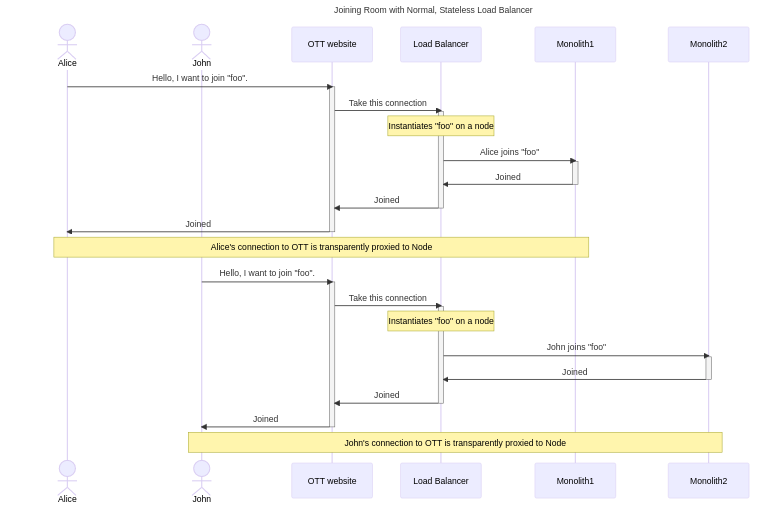
\includegraphics{Figures/join-room-stateless.png}}
  \caption{\label{Figure::join-room-stateless} Sequence Diagram for Room Loading on Stateless Balancer.}
\end{figure}


\section{Balancer Must Use Asynchronous I/O \index{async} \index{asynchronous I/O} \index{io}}

The Balancer's workload is I/O bound, and it must be able to handle many concurrent network connections. For I/O bound workloads, it's more performant to use asynchronous I/O\cite{async-vs-threads}.
